\documentclass[a4paper,10pt]{article}
\usepackage[T2A]{fontenc}
\usepackage[utf8]{inputenc}%включаем свою кодировку: koi8-r или utf8 в UNIX, cp1251 в 
\usepackage[english,russian]{babel}%используем русский и английский языки с переносами
\usepackage{amssymb,amsfonts,amsmath,mathtext,cite,enumerate,float,bm,hyperref}
\usepackage{geometry}
\geometry{left=1cm}
\geometry{right=1cm}
\geometry{top=1cm}
\geometry{bottom=2cm}
\usepackage{tikz}
\allowdisplaybreaks

\setlength{\parindent}{0cm}
\begin{document}
\tableofcontents
\clearpage

%\documentclass[a4paper,10pt]{article} %размер бумаги устанавливаем А4, шрифт 12пунктов
\usepackage[T2A]{fontenc}
\usepackage[utf8]{inputenc}%включаем свою кодировку: koi8-r или utf8 в UNIX, cp1251 в 
\usepackage[english,russian]{babel}
\usepackage{amssymb,amsfonts,amsmath,mathtext,cite,enumerate,float}
\usepackage{hyperref}
\renewcommand{\rmdefault}{ftm}

\usepackage{geometry}
\geometry{left=1cm}
\geometry{right=1cm}
\geometry{top=1cm}
\geometry{bottom=1cm}

\begin{document}
	
	Вспомним что:
	$$
		\sin x = A x \prod\limits_{n = 1}^{\infty} \left(1 - \frac{x^2}{\pi^2 n^2}\right) =
		A x \left[
		1 -
		\frac{x^2}{\pi^2} \left(1 + \frac{1}{2^2} + \frac{1}{3^2} + \ldots \right) +
		\frac{x^4}{\pi^4} \alpha_4 + 
		\frac{x^6}{\pi^6} \alpha_6 + \ldots
		\right]
	$$
	Теперь:
	$$
		\sin x = x - \frac{x^3}{6} + \frac{x^5}{120} - \ldots
	$$
	и финт ушами:
	$$
		\left(1 + \frac{1}{2^2} + \frac{1}{3^2} + \ldots \right)^2 = 
		1 + \frac{1}{2^4} + \frac{1}{3^4} + \ldots + 2 \alpha_4
	$$
	Ба-бах:
	$$
		1 + \frac{1}{2^4} + \frac{1}{3^4} + \ldots = \frac{\pi^4}{36} - 2 \frac{\pi^4}{120} = \frac{\pi^4}{90}
	$$

\end{document}

%\section{Сферические координаты}

Связь декартовых $(x, y, z)$ и сферических координат $(r, \theta, \alpha)$ даётся выражениями:
\[
	\begin{aligned}
		& x = r \sin \theta \cos \alpha \\
		& y = r \sin \theta \sin \alpha \\
		& z = r \cos \theta 
	\end{aligned}
\]
Орты сферической системы координат найдём из соотношений:
\[
	\begin{aligned}
	& \left|\frac{\partial \vec{r}}{\partial r}\right| \vec{e}_r = \frac{\partial \vec{r}}{\partial r} =  \sin \theta \cos \alpha\, \vec{e}_x + \sin \theta \sin \alpha\, \vec{e}_y + \cos \theta\, \vec{e}_z \\
	& \left|\frac{\partial \vec{r}}{\partial \theta}\right| \vec{e}_\theta = \frac{\partial \vec{r}}{\partial \theta} =  r \cos \theta \cos \alpha\, \vec{e}_x + r \cos \theta \sin \alpha\, \vec{e}_y - r \sin \theta\, \vec{e}_z \\
	& \left|\frac{\partial \vec{r}}{\partial \alpha}\right| \vec{e}_\alpha = \frac{\partial \vec{r}}{\partial \alpha} = - r \sin \theta \sin \alpha\, \vec{e}_x + r \sin \theta \cos \alpha\, \vec{e}_y
	\end{aligned}
\]
Коэффициенты Ламе:
\[
	\begin{aligned}
		& H_r =  \left|\frac{\partial \vec{r}}{\partial r}\right| = 1 \\
		& H_\theta = \left|\frac{\partial \vec{r}}{\partial \theta}\right| = r \\
		& H_\alpha = \left|\frac{\partial \vec{r}}{\partial \alpha}\right| = r \sin \theta
	\end{aligned}
\]
Орты
\[
	\begin{aligned}
	& \vec{e}_r = \sin \theta \cos \alpha\, \vec{e}_x + \sin \theta \sin \alpha\, \vec{e}_y + \cos \theta\, \vec{e}_z \\
	& \vec{e}_\theta = \cos \theta \cos \alpha\, \vec{e}_x + \cos \theta \sin \alpha\, \vec{e}_y - \sin \theta\, \vec{e}_z \\
	& \vec{e}_\alpha = -\sin \alpha\, \vec{e}_x + \cos \alpha\, \vec{e}_y
	\end{aligned}
\]
Орты декартовой системы, выраженные через орты сферической системы:
\[
	\begin{aligned}
	& \vec{e}_x = \sin \theta \cos \alpha\, \vec{e}_r + \cos \theta \cos \alpha\, \vec{e}_\theta -\sin \alpha\,  \vec{e}_\alpha \\
	& \vec{e}_y = \sin \theta \sin \alpha\, \vec{e}_r + \cos \theta \sin \alpha\, \vec{e}_\theta + \cos \alpha\, \vec{e}_\alpha \\
	& \vec{e}_z = \cos \theta\,\vec{e}_r - \sin \theta\, \vec{e}_\theta
	\end{aligned}
\]
Немного о производных от ортов (для вывода нужно помнить, что орты декартовой системы образуют базис, не зависящий от его положения, в то время как орты сферической системы образуют базис, который меняется от точки к точке):
\[
	\begin{aligned}
	& \frac{\partial \vec{e}_r}{\partial r} = 0 \\
	& \frac{\partial \vec{e}_r}{\partial \theta} = \vec{e}_\theta \\
	& \frac{\partial \vec{e}_r}{\partial \alpha} = \sin \theta\, \vec{e}_\alpha
	\end{aligned}
	\quad
	\begin{aligned}
	& \frac{\partial \vec{e}_\theta}{\partial r} = 0 \\
	& \frac{\partial \vec{e}_\theta}{\partial \theta} = -\vec{e}_r \\
	& \frac{\partial \vec{e}_\theta}{\partial \alpha} = \cos \theta\, \vec{e}_\alpha
	\end{aligned}
	\quad
	\begin{aligned}
	& \frac{\partial \vec{e}_\alpha}{\partial r} = 0 \\
	& \frac{\partial \vec{e}_\alpha}{\partial \theta} = 0 \\
	& \frac{\partial \vec{e}_\alpha}{\partial \alpha} = -\sin\theta \, \vec{e}_r -\cos \theta\, \vec{e}_\theta
	\end{aligned}
\]

%\section{Волновые функции в $p$ и $x$ представлениях}

Для описания квантовых процессов вводят волновые функции, которые являются суперпозициями волн д'Бройля. Для одной частицы:
\[
	\psi(\vec{r}, t) = A \int C_(\vec{p}, t) \exp \left(\frac{i}{\hbar} \vec{p} \cdot \vec{r}\right) d^3p
\]
\[
	C(\vec{p}, t) = B \int \psi(\vec{r}, t) \exp \left(-\frac{i}{\hbar} \vec{p} \cdot \vec{r}\right) d^3r
\]
$\psi(\vec{r}, t)$ -- волновая функция в $x$ представлении. $C(\vec{p}, t)$ -- волновая функция в $p$ представлении. $A$ и $B$ -- действительные числа, которые можно найти из условия нормировки. Нормировка:
\[
	\int \psi^*(\vec{r}, t) \psi(\vec{r}, t) d^3r = \int C^*(\vec{p}, t) C(\vec{p}, t) d^3p = 1
\]
\[
	\begin{gathered}
		A^2\iint C^*(\vec{p'}, t) C(\vec{p}, t) \exp \left(\frac{i}{\hbar} (\vec{p'} - \vec{p}) \cdot \vec{r}\right) d^3p\, d^3p'\, d^3r 
		= \\
		=
		A^2\int C^*(\vec{p'}, t) C(\vec{p}, t) (2\pi \hbar)^3 \delta(\vec{p'} - \vec{p}) d^3p\, d^3p'
		= \\
		=
		A^2 (2\pi \hbar)^3 \int C^*(\vec{p}, t) C(\vec{p}, t) d^3p = A^2 (2\pi \hbar)^3 = 1
	\end{gathered}
\]
\[
	\begin{gathered}
		B^2\iint \psi^*(\vec{r'}, t) \psi(\vec{r}, t) \exp \left(\frac{i}{\hbar} \vec{p} \cdot (\vec{r'} - \vec{r})\right) d^3p \, d^3r \, d^3r'
		= \\
		=
		B^2 (2\pi\hbar)^3 \iint \psi^*(\vec{r'}, t) \psi(\vec{r}, t) \delta(\vec{r'} - \vec{r}) d^3r \, d^3r' = B^2 (2\pi\hbar)^3 \iint \psi^*(\vec{r}, t) \psi(\vec{r}, t) d^3r 
		= \\
		=
		B^2 (2\pi\hbar)^3 = 1
	\end{gathered}
\]
\[
	A = B =\frac{1}{(2\pi\hbar)^{3/2}}
\]
Обратимость непосредственно следует из обратимости преобразования Фурье.

\section{Оператор импульса в $x$ представлении}
Оператор импульса в $p$ представлении, просто вектор $\vec{p}$. 
По определению оператор импульса $\hat{\vec{p}}$ в $x$ представлении:
\[
	\langle \vec{p} \,\rangle = \int \psi^*(\vec{r}, t) \hat{\vec{p}} \psi(\vec{r}, t) d^3r
\]
Средний импульс:
\[
	\begin{gathered}
	\langle \vec{p} \,\rangle = 
	\int C^*(\vec{p}, t) \vec{p} C(\vec{p}, t) d^3p = \\ =
	\frac{1}{(2\pi\hbar)^{3}} \iiint \vec{p} \psi^*(\vec{r'}, t) \psi(\vec{r}, t) \exp \left(\frac{i}{\hbar} \vec{p} \cdot (\vec{r'} - \vec{r})\right) d^3r'\, d^3r\, d^3p = \\ =
	\frac{1}{(2\pi\hbar)^{3}} \iint \psi^*(\vec{r'}, t) \psi(\vec{r}, t) \frac{\hbar}{i}\frac{\partial}{\partial \vec{r'}}\int\exp \left(\frac{i}{\hbar} \vec{p} \cdot (\vec{r'} - \vec{r})\right) d^3p\, d^3r'\, d^3r = \\ =
	\iint \psi^*(\vec{r'}, t) \psi(\vec{r}, t) \frac{\hbar}{i} \frac{\partial}{\partial \vec{r'}} \delta(\vec{r'} - \vec{r}) d^3r'\, d^3r = \\ =
	[\text{интегрируем по частям и учитываем, что $\psi = 0$ на $\infty$}] =
	\end{gathered}
\]
\[
	\begin{gathered}
	= - \frac{\hbar}{i} \iint \delta(\vec{r'} - \vec{r}) \frac{\partial}{\partial \vec{r'}} \psi^*(\vec{r'}, t) \psi(\vec{r}, t) d^3r'\, d^3r = \\ =
	- \frac{\hbar}{i} \int \psi(\vec{r}, t) \frac{\partial}{\partial \vec{r}} \psi^*(\vec{r}, t) d^3r = \\ =
	[\text{ещё одно интегрирование по частям}] = \\ =
	\frac{\hbar}{i} \int \psi^*(\vec{r}, t) \frac{\partial}{\partial \vec{r}} \psi(\vec{r}, t) d^3r
	\end{gathered}
\]
\[
	\hat{\vec{p}} = \frac{\hbar}{i} \frac{\partial}{\partial \vec{r}} = - i \hbar \frac{\partial}{\partial \vec{r}}
\]

\section{Оператор координаты в $p$ представлении}
Оператор координаты в $x$ представлении $\vec{r}$. В $p$ представлении по определению:
\[
	\langle \vec{r}\,\rangle = \int C^*(\vec{p}, t) \hat{\vec{r}} C(\vec{p}, t) d^3p	
\]
Итак:
\[
	\begin{gathered}
	\langle \vec{r}\,\rangle = \int \psi^*(\vec{r}, t) \vec{r} \psi(\vec{r}, t) d^3 r = \\ =
	\frac{1}{(2\pi\hbar)^{3}} \iiint C^*(\vec{p'}, t) C(\vec{p}, t) \vec{r} 
	\exp 
	\left(
		-\frac{i}{\hbar}
			(\vec{p'} - \vec{p})\cdot \vec{r}
	\right) d^3r\,d^3p\,d^3p' =
	\\ =
	\frac{1}{(2\pi\hbar)^{3}} \iint C^*(\vec{p'}, t) C(\vec{p}, t)
	\frac{\hbar}{i}
	\frac{\partial}{\partial \vec{p}}
	\int
	\exp 
	\left(
		\frac{i}{\hbar}
		(\vec{p} - \vec{p'})\cdot \vec{r}
	\right) d^3r\,d^3p\,d^3p' = 
	\\ =
	\frac{\hbar}{i}\iint C^*(\vec{p'}, t) C(\vec{p}, t)
	\frac{\partial}{\partial \vec{p}}
	\delta(\vec{p} - \vec{p'}) d^3p\, d^3p'
	= \\ =
	[\text{интегрируем по частям и учитываем, что $C = 0$ на $\infty$}] = \\ =
	-\frac{\hbar}{i}
	\iint 
	C^*(\vec{p}, t)
	\frac{\partial}{\partial \vec{p}}
	C(\vec{p}, t)
	d^3p
	\end{gathered}
\]
В результате:
\[
	\hat{\vec{r}} = 
	-\frac{\hbar}{i} \frac{\partial}{\partial \vec{p}} =
	i\hbar \frac{\partial}{\partial \vec{p}} 
\]
Уравнение Шрёдингера сохраняет свою форму:
\[
	\sum_{i=1}^N\frac{p_i^2}{2m_i} C + \hat{U}\left(i \hbar \frac{\partial}{\partial p_1}, \ldots, i \hbar \frac{\partial}{\partial p_N}\right) C = i\hbar \frac{\partial C}{\partial t}
\]
%\section{Определение и некоторые свойства функций Эйри}

Функциями Эйри называют:
\[
	\mathrm{Ai\,}(x) = \frac{1}{\pi} \int\limits_0^\infty \cos \left( \frac{t^3}{3} + xt\right) dt
\]
\[
	\mathrm{Bi\,}(x) = \frac{1}{\pi} \int\limits_0^\infty \left[e^{-\frac{1}{3}t^3 - xt} + \sin \left( \frac{t^3}{3} + xt\right)\right] dt
\]
Асимптотика (можно найти, проинтегрировав методом перевала в комплексной плоскости):
\[
	\mathrm{Ai\,}(x) \underset{x \to \infty}{\approx} \frac{1}{2\sqrt{\pi} x^{1/4}} \exp \left( -\frac{2}{3} x^{3/2}\right)
\]
\[
	\mathrm{Bi\,}(x) \underset{x \to \infty}{\approx} \frac{1}{\sqrt{\pi} x^{1/4}} \exp \left( \frac{2}{3} x^{3/2}\right)
\]
\[
	\mathrm{Ai\,}(x) \underset{x \to -\infty}{\approx} \frac{1}{\sqrt{\pi} x^{1/4}} \sin \left( \frac{2}{3} |x|^{3/2} + \frac{\pi}{4}\right)
\]
\[
	\mathrm{Bi\,}(x) \underset{x \to -\infty}{\approx} \frac{1}{\sqrt{\pi} x^{1/4}} \cos \left( \frac{2}{3} |x|^{3/2}+ \frac{\pi}{4}\right)
\]
Интеграл (легко находится с использованием дельта функции)
\[
	\int\limits_{-\infty}^{\infty} \mathrm{Ai\,}(x)\, dx = 1
\]
Функции Эйри удовлетворяют уравнению Эйри:
\[
	u'' - xu = 0
\]
Рассмотрим интеграл:
\[
	\int\limits_{a}^{\infty}\mathrm{\,Ai\,}'(x) \mathrm{\,Ai\,}''(x) dx= 
	\int\limits_{a}^{\infty} x \mathrm{\,Ai\,}'(x) \mathrm{\,Ai\,}(x) dx
\]
\[
	\Rightarrow \frac{\left[\mathrm{\,Ai\,}'(x) \right]^2}{2} \Bigg|_{a}^{\infty} =
	x \frac{\left[\mathrm{\,Ai\,}(x) \right]^2}{2} \Bigg|_{a}^{\infty} - 
	\int\limits_{a}^{\infty} \frac{\left[\mathrm{\,Ai\,}(x) \right]^2}{2} dx
\]
Откуда следует весьма важный интеграл:
\[
	\int\limits_{a}^{\infty} \left[\mathrm{\,Ai\,}(x) \right]^2 dx =
	\left[\mathrm{\,Ai\,}'(a) \right]^2  - a \left[\mathrm{\,Ai\,}(a) \right]^2
\]

%\section{Решение линейных уравнений}

Поставим следующую задачу:
\[
	L\left[y\right] = \frac{\partial y}{\partial t} 
\]
\[
	y(x, t)\Big|_{t = 0} = y(x, 0) 
\]
$L$ -- произвольный линейный оператор.
Пусть собственные значения $Y(x, \lambda)$ удовлетворяет уравнению:
\[
	L\left[Y\right] = \lambda Y
\]
и если спектр $\lambda$ сплошной, существует функция $Y^{-1}(x, \lambda')$, такая что:
\[
	\int\limits_{-\infty}^{\infty} Y^{-1}(x, \lambda') Y(x, \lambda) dx = \delta(\lambda - \lambda')
\]
Будем искать $y$ в виде:
\[
	y = \int\limits_{-\infty}^{\infty} A(\lambda) e^{\lambda t} Y(x, \lambda)\, d\lambda
\]
Простой подстановкой можно проверить, что это выражение в самом деле является решением уравнения. $A(\lambda)$ определим из начальных условий:
\[
	y(x, 0) = \int\limits_{-\infty}^{\infty} A(\lambda) Y(x, \lambda)\, d\lambda
\]
\[
	A(\lambda) = \int\limits_{-\infty}^{\infty} y(x, 0) Y^{-1}(x, \lambda)\, dx
\]
Подставляем в решение и получаем:
\[
	y(x, t) = \int\limits_{-\infty}^{\infty} y(x', 0) \int\limits_{-\infty}^{\infty} e^{\lambda t}Y^{-1}(x', \lambda) Y(x, \lambda)\, d\lambda\, dx'
\]

\section{Решение линейных уравнений в случае дискретного спектра}

В случае дискретного спектра у нас есть система функций:
\[
	Y_1(x), Y_2(x), \ldots, Y_n(x), \ldots
\]
и соответствующая ей последовательность чисел:
\[
	\lambda_1, \lambda_2, \ldots
\]
Если удалось построить дополнительную систему функций
\[
	Y_1^{-1}(x), Y_2^{-1}(x), \ldots, Y_n^{-1}(x), \ldots
\]
такую что
\[
	\int\limits_{-\infty}^{\infty} Y_k^{-1}(x) Y_n(x) dx = \delta_{kn}
\]
То решение уравнения можно найти в виде:
\[
	y = \sum_{k=1}^{\infty} A_k e^{\lambda_k t} Y_k(x)
\]
\[
	A_k = \int\limits_{-\infty}^{\infty} Y_k^{-1}(x) y(x, 0) dx
\]
Получаем окончательно решение:
\[
	y(x, t) = \int\limits_{-\infty}^{\infty} y(x', 0) \sum_{k=1}^{\infty} e^{\lambda_k t} Y_k^{-1}(x') Y_k(x) dx'
\]
%\section{Частица в однородном силовом поле}

Пусть сила, действующая на частицу, равна $F$ по модулю и направлена вдоль оси $z$ в обратном направлении. Гамильтониан в классическом случае:
\[
	\hat{H} = \frac{\hat{p}_z^2}{2m} + F \hat{z} 
\]
Уравнение Шрёдингера:
\[
	\frac{p_z^2}{2m} C(p_z, t) + i \hbar F \frac{\partial C(p_z, t)}{\partial p_z} = i\hbar \frac{\partial C(p_z, t)}{\partial t}
\]
Вместо $\lambda$ будет выступать $-iE/\hbar$. Для $Y$ получаем уравнение
\[
	\frac{p_z^2}{2m} Y + i \hbar F \frac{\partial Y}{\partial p_z} = E Y
\]
Будем искать $Y$ в форме $\exp f(p_z)$:
\[
	i \hbar F \frac{\partial f(p_z)}{\partial p_z} = E - \frac{p_z^2}{2m}
\]
\[
	f(p_z) = - i \frac{E}{\hbar F} p_z + i \frac{1}{6 m \hbar F} p_z^3 + const
\]
Константа уйдёт в нормировочный множитель. 
\[
	Y(p_z, E) = A \exp \left(-\frac{i}{\hbar} \left( \frac{E}{F} p_z - \frac{1}{6 m F} p_z^3 \right) \right)
\]
\[
	Y^{-1}(p_z, E) = B \exp \left(\frac{i}{\hbar} \left( \frac{E}{F} p_z - \frac{1}{6 m F} p_z^3 \right) \right)
\]
\[
	AB \int\limits_{-\infty}^{\infty} \exp \left(\frac{i p_z}{\hbar F} (E' - E) \right) dp_z = 
	2\pi AB\hbar F\, \delta(E' - E) = \delta(E' - E)
\]
Откуда можно в качестве $A$ и $B$ можно взять константы:
\[
	A = B = \frac{1}{\sqrt{2\pi \hbar F}}
\]
\[
	\begin{gathered}
		C(p_z, t) = \int\limits_{-\infty}^{\infty} C(p_z, 0) \int\limits_{-\infty}^{\infty} AB
		\exp \left(-\frac{i}{\hbar} \left( E \left(\frac{p_z - p_z'}{F} + t\right) - \frac{1}{6 m F} (p_z^3 - p_z'^3) \right)
		\right)\, dE\, dp_z' = \\
		=
		\int\limits_{-\infty}^{\infty} C(p_z', 0) \delta(p_z - p_z' + F t) 
		\exp \left(\frac{i}{6 m \hbar F} (p_z^3 - p_z'^3) \right)
		\, dp_z' = \\
		=
		C(p_z + F t, 0) \exp \left(\frac{i(-3 p_z^2 F t - 3 p_z F^2 t^2 - F^3 t^3)}{6 m \hbar F} \right) = \\
		=
		C(p_z + F t, 0) \exp \left(-\frac{i}{\hbar} \left(\frac{p_z^2}{2m} t + \frac{p_z F t^2}{2 m} + \frac{F^2 t^3}{6 m}\right) \right)
	\end{gathered}
\]
Чтобы получить дискретный спектр нужно ввести дополнительные условия. Чаще всего таким условием выступает поверхность, за пределы которой частица не может попасть. В качестве такой поверхности может выступать поверхность Земли для поля тяжести, обкладка конденсатора.

\section{Гауссовский волновой пакет в однородном поле}

Пусть
\[
	\psi(z, 0) = \frac{1}{\sqrt[4]{2\pi \sigma^2}} \exp \left( -\frac{(z - z_0)^2}{4\sigma^2}\right)
\]
\[
	\begin{gathered}
		C(p_z, 0) = \frac{1}{\sqrt[4]{2\pi \sigma^2}}\frac{1}{(2\pi\hbar)^{1/2}} \int\limits_{-\infty}^{\infty} \exp \left(-\frac{(z - z_0)^2}{4\sigma^2} - \frac{i}{\hbar} p_z z  \right) dz = \\
		=
		\frac{1}{\sqrt[4]{2\pi \sigma^2}}\frac{1}{(2\pi\hbar)^{1/2}} \exp\left(-\frac{i}{\hbar}p_z z_0\right)\int\limits_{-\infty}^{\infty} \exp \left(-\frac{(z - z_0)^2}{4\sigma^2} - \frac{i}{\hbar} p_z (z - z_0)  \right) dz = \\
		=
		\frac{1}{\sqrt[4]{2\pi \sigma^2}}\frac{1}{(2\pi\hbar)^{1/2}} \exp\left(-\frac{i}{\hbar}p_z z_0\right)
		\int\limits_{-\infty}^{\infty} \exp \left(-\frac{(z - z_0)^2}{4\sigma^2} - 2 \frac{i}{\hbar} \sigma p_z \frac{(z - z_0)}{2 \sigma}  \right) dz = \\
		=
		\frac{1}{\sqrt[4]{2\pi \sigma^2}}\frac{1}{(2\pi\hbar)^{1/2}} \exp\left(-\frac{i}{\hbar}p_z z_0\right)
		\int\limits_{-\infty}^{\infty} \exp \left(-\left(\frac{(z - z_0)}{2 \sigma} + \frac{i}{\hbar} \sigma p_z \right)^2 - \frac{\sigma^2 p_z^2}{\hbar^2}  \right) dz = \\
		=
		\frac{2\sqrt[4]{2\pi \sigma^2}}{(2\pi\hbar)^{1/2}} \exp\left(-\frac{i}{\hbar}p_z z_0 - \frac{\sigma^2 p_z^2}{\hbar^2} \right) = \\
		=
		\sqrt[4]{\frac{2\sigma^2}{\pi \hbar^2}} \exp\left(-\frac{i}{\hbar}p_z z_0 - \frac{\sigma^2 p_z^2}{\hbar^2} \right)
	\end{gathered}
\]
\[
	\begin{gathered}
		\langle z \rangle =
		\sqrt{\frac{2\sigma^2}{\pi \hbar^2}} 
		\int\limits_{-\infty}^{\infty} \left(z_0 - \frac{2i\hbar \sigma^2}{\hbar^2} (p_z + Ft) + \frac{p_z}{m} t +  \frac{F t^2}{2m}\right) 
		\exp\left( - \frac{2\sigma^2 (p_z + Ft)^2}{\hbar^2} \right) dp_z = \\
		=
		\sqrt{\frac{2\sigma^2}{\pi \hbar^2}} 
		\int\limits_{-\infty}^{\infty} \left(z_0 - \frac{2i\hbar \sigma^2}{\hbar^2} (p_z + Ft) + \frac{p_z + F t}{m} t -  \frac{F t^2}{2m}\right) 
		\exp\left( - \frac{2\sigma^2 (p_z + Ft)^2}{\hbar^2} \right) dp_z = \\
		=
		z_0 - \frac{F t^2}{2m}	
	\end{gathered}
\]
\[
	\begin{gathered}
		\langle z^2 \rangle =
		\sqrt{\frac{2\sigma^2}{\pi \hbar^2}} 
		\int\limits_{-\infty}^{\infty} \left(z_0 - \frac{F t^2}{2m} + \left(\frac{t}{m}- 2\frac{i \sigma^2}{\hbar}\right) (p_z + Ft)\right)^2
		\exp\left( - \frac{2\sigma^2 (p_z + Ft)^2}{\hbar^2} \right) dp_z + \\
		+
		\sqrt{\frac{2\sigma^2}{\pi \hbar^2}} 
		\int\limits_{-\infty}^{\infty} \left(2\sigma^2 + \frac{i\hbar}{m} t \right)
		\exp\left( - \frac{2\sigma^2 (p_z + Ft)^2}{\hbar^2} \right) dp_z = \\
		=
		\left(z_0 - \frac{F t^2}{2m}\right)^2 +
		\left(\frac{t}{m}- 
		2\frac{i \sigma^2}{\hbar}\right)^2 \frac{\hbar^2}{4 \sigma^2} +
		\left(2\sigma^2 + \frac{i\hbar}{m} t \right) = \\
		=
		\left(z_0 - \frac{F t^2}{2m}\right)^2 +
		\frac{t^2\hbar^2}{4 m^2 \sigma^2} + \sigma^2
	\end{gathered}
\]
Дисперсия:
\[
	\langle z^2 \rangle - \langle z \rangle^2 =
	\frac{t^2\hbar^2}{4 m^2 \sigma^2} + \sigma^2
\]

\section{Частица в однородном поле над непроницаемым барьером}

Рассмотрим частицу в треугольной потенциальной яме:

\parbox{\textwidth}{
	\centering
\begin{tikzpicture}[>= stealth]
\draw[->] (0, -0.2) -- (0, 3) node[left]{$U$};
\draw[->] (-0.2, 0) -- (3, 0) node[below]{$z$};
\draw[line width = 2pt] (0, 0) node[above left]{$0$} -- (0, 2.5);
\draw[line width = 2pt] (0, 0) -- (2.5, 2.5) node[below right]{$F z$}; 
\end{tikzpicture}
}
В этом случае спектр дискретный. Нам необходимо от импульсной формы перейти к координатной. В этом случае получится обычное стационарное уравнение Шрёдингера c решением:
\[
	\begin{gathered}
	\psi(z, E) = \int\limits_{-\infty}^{\infty} 
	A \exp \left(-\frac{i}{\hbar} \left( \frac{E - Fz}{F} p_z - \frac{1}{6 m F} p_z^3 \right) \right) dp_z = \\ =
	\int\limits_{-\infty}^{\infty} 
	A \cos \left( -\frac{E - Fz}{F \hbar} p_z + \frac{1}{2 m F \hbar} \frac{p_z^3}{3} \right) dp_z
	= \\ =
	A (2 m F \hbar)^{1/3} \mathrm{\,Ai\,} \left((2 m F \hbar)^{1/3}\frac{Fz - E}{F \hbar}\right)	
	\end{gathered}
\]
Зная корни функции Эйри $x_1, x_2, \ldots$, легко найти спектр:
\[
	E_k = - (2 m)^{-1/3} \hbar^{2/3} F^{2/3} x_k
\]
А воспользовавшись интегралом:
\[
	\int\limits_{x_k}^{\infty} \mathrm{\,Ai\,}^2 (x)\,dx = \left[\mathrm{\,Ai\,}' (x_k)\right]^2,
\]
нормировочную константу:
\[
	A = \hbar^{-2/3} (2 m F)^{-1/6} |\mathrm{\,Ai\,}' (x_k)|^{-1}
\]
Окончательно волновые функции:
\[
	\psi_k(z) = \frac{(2mF)^{1/6}}{\hbar^{1/3}|\mathrm{\,Ai\,}' (x_k)|} \mathrm{\,Ai\,} \left((2 m F \hbar)^{1/3} \frac{z}{\hbar} + x_k \right)
\]
Для электронов:
\[
	E_k \approx -1{,}14\times10^{6} F^{2/3} x_k \text{ эВ}
\]
Найдём количество значений $x_k$ приходящихся на интервал $(k_{b}T, k_{b}(T + \Delta T))$ при $\Delta T= 10 $К и $T = 300 $К (обозначим эту величину $N$) для поля силы тяжести, что соответствует частице над поверхностью Земли. Для этого воспользуемся приближённым выражением:
\[
	\mathrm{Ai\,}(x) \underset{x \to -\infty}{\approx} \frac{1}{\sqrt{\pi} x^{1/4}} \sin \left( \frac{2}{3} |x|^{3/2} + \frac{\pi}{4}\right)
\]
\[
	|x_k|^{3/2} \approx \frac{3}{2}\pi k - \frac{3\pi}{8}
\]
\[
	N \approx \frac{2^{3/2}}{3\pi g \hbar m^{1/2}} k_{b}^{3/2} T^{3/2} ((1 + \Delta T/T)^{3/2} - 1) \approx 
	\frac{2^{1/2}}{\pi g \hbar m^{1/2}} k_{b}^{3/2} T^{1/2} \Delta T
\]
Для электронов:
\[
	N \approx 4{,}07\times10^{15}
\]
Далее можно приближённо вычислить среднюю температуру таких частиц и так далее.
%\section{Оператор импульса в сферических координатах и коммутационные соотношения}

Нам известно, что оператор импульса это градиент с коэффициентом. Градиент в сферических координатах:
\[
	\nabla = \left\{\frac{\partial}{\partial r}, \frac{1}{r}\frac{\partial}{\partial \theta}, \frac{1}{r \sin \theta}\frac{\partial}{\partial \alpha} \right\}
\]
Оператор Лапласа, который фигурирует в уравнении Шрёдингера:
\[
	\Delta = \nabla \cdot \nabla = \frac{\partial^2}{\partial r^2} + \frac{1}{r^2}\frac{\partial^2}{\partial \theta^2} +\frac{1}{r^2 \sin^2 \theta}\frac{\partial^2}{\partial \alpha^2}
\]
Но умные люди давно подсчитали, что:
\[
	\Delta = 
	\frac{1}{r^2}\frac{\partial}{\partial r} \left(r^2 \frac{\partial}{\partial r}\right)
	+ \frac{1}{r^2 \sin \theta} \frac{\partial}{\partial \theta} \left(\sin \theta \frac{\partial}{\partial \theta}\right)
	+ \frac{1}{r^2 \sin^2 \theta} \frac{\partial^2}{\partial \alpha^2}
\]
и результаты, вообще говоря, не совпадают. Где мы ошиблись? Ответ на этот вопрос чрезвычайно прост: мы не должны были забывать об ортах. Запишем градиент иначе:
\[
	\nabla = \vec{e}_r \frac{\partial}{\partial r} + \vec{e}_\theta \frac{1}{r}\frac{\partial}{\partial \theta} + \vec{e}_\alpha \frac{1}{r \sin \theta}\frac{\partial}{\partial \alpha}
\]
И воспользуемся формулами:
\[
\begin{aligned}
& \frac{\partial \vec{e}_r}{\partial r} = 0 \\
& \frac{\partial \vec{e}_r}{\partial \theta} = \vec{e}_\theta \\
& \frac{\partial \vec{e}_r}{\partial \alpha} = \sin \theta\, \vec{e}_\alpha
\end{aligned}
\quad
\begin{aligned}
& \frac{\partial \vec{e}_\theta}{\partial r} = 0 \\
& \frac{\partial \vec{e}_\theta}{\partial \theta} = -\vec{e}_r \\
& \frac{\partial \vec{e}_\theta}{\partial \alpha} = \cos \theta\, \vec{e}_\alpha
\end{aligned}
\quad
\begin{aligned}
& \frac{\partial \vec{e}_\alpha}{\partial r} = 0 \\
& \frac{\partial \vec{e}_\alpha}{\partial \theta} = 0 \\
& \frac{\partial \vec{e}_\alpha}{\partial \alpha} = -\sin\theta \, \vec{e}_r -\cos \theta\, \vec{e}_\theta
\end{aligned}
\]
Тогда
\[
	\begin{gathered}
		\Delta = 
		\vec{e}_r\cdot \frac{\partial}{\partial r} 
		\left(\vec{e}_r \frac{\partial}{\partial r} + \vec{e}_\theta \frac{1}{r}\frac{\partial}{\partial \theta} + \vec{e}_\alpha \frac{1}{r \sin \theta}\frac{\partial}{\partial \alpha}\right)
		+ \\ +
		\vec{e}_\theta\cdot \frac{1}{r}\frac{\partial}{\partial \theta}
		\left(\vec{e}_r \frac{\partial}{\partial r} + \vec{e}_\theta \frac{1}{r}\frac{\partial}{\partial \theta} + \vec{e}_\alpha \frac{1}{r \sin \theta}\frac{\partial}{\partial \alpha}\right)
		+
		\vec{e}_\alpha\cdot \frac{1}{r \sin \theta}\frac{\partial}{\partial \alpha}
		\left(\vec{e}_r \frac{\partial}{\partial r} + \vec{e}_\theta \frac{1}{r}\frac{\partial}{\partial \theta} + \vec{e}_\alpha \frac{1}{r \sin \theta}\frac{\partial}{\partial \alpha}\right) 
		= \\ =
		\frac{\partial^2}{\partial r^2} +
		\frac{1}{r} \frac{\partial}{\partial r} +
		\frac{1}{r^2} \frac{\partial^2}{\partial \theta^2} +
		\frac{1}{r} \frac{\partial}{\partial r} +
		\frac{1}{r^2} \frac{\cos \theta}{\sin \theta} \frac{\partial}{\partial \theta} +
		\frac{1}{r^2 \sin^2 \theta} \frac{\partial^2}{\partial \alpha^2}
		= \\ =
		\frac{1}{r^2}\frac{\partial}{\partial r} \left(r^2 \frac{\partial}{\partial r}\right)
		+ \frac{1}{r^2 \sin \theta} \frac{\partial}{\partial \theta} \left(\sin \theta \frac{\partial}{\partial \theta}\right)
		+ \frac{1}{r^2 \sin^2 \theta} \frac{\partial^2}{\partial \alpha^2}
	\end{gathered}
\]
Итак, оператор импульса в сферических координатах:
\[
	\hat{\vec{p}} = -i\hbar \left(\vec{e}_r \frac{\partial}{\partial r} + \vec{e}_\theta \frac{1}{r}\frac{\partial}{\partial \theta} + \vec{e}_\alpha \frac{1}{r \sin \theta}\frac{\partial}{\partial \alpha} \right)
\]
Соотношения коммутации в случае декартовых координат:
\[
	[\hat{p}_i, \hat{p}_j] = \hat{p}_i \hat{p}_j - \hat{p}_j \hat{p}_i = 0
\]
С точки зрения векторов это означает, что в терминах полного произведения векторов матрица $\hat{\vec{p}}\hat{\vec{p}}$ симметрична.
\[
	\begin{gathered}
	\nabla\nabla = 
	\vec{e}_r \frac{\partial}{\partial r} 
	\left(\vec{e}_r \frac{\partial}{\partial r} + \vec{e}_\theta \frac{1}{r}\frac{\partial}{\partial \theta} + \vec{e}_\alpha \frac{1}{r \sin \theta}\frac{\partial}{\partial \alpha}\right)
	+ \\ +
	\vec{e}_\theta \frac{1}{r}\frac{\partial}{\partial \theta}
	\left(\vec{e}_r \frac{\partial}{\partial r} + \vec{e}_\theta \frac{1}{r}\frac{\partial}{\partial \theta} + \vec{e}_\alpha \frac{1}{r \sin \theta}\frac{\partial}{\partial \alpha}\right)
	+
	\vec{e}_\alpha \frac{1}{r \sin \theta}\frac{\partial}{\partial \alpha}
	\left(\vec{e}_r \frac{\partial}{\partial r} + \vec{e}_\theta \frac{1}{r}\frac{\partial}{\partial \theta} + \vec{e}_\alpha \frac{1}{r \sin \theta}\frac{\partial}{\partial \alpha}\right) 
	= \\ =
	\vec{e}_r \vec{e}_r \frac{\partial^2}{\partial r^2} +
	\vec{e}_r \vec{e}_\theta \frac{\partial}{\partial r} \frac{1}{r}\frac{\partial}{\partial \theta} +
	\vec{e}_r \vec{e}_\alpha \frac{\partial}{\partial r} \frac{1}{r \sin \theta}\frac{\partial}{\partial \alpha} +
	\vec{e}_\theta \vec{e}_r \left(\frac{1}{r} \frac{\partial^2}{\partial \theta\, \partial r} - \frac{1}{r^2} \frac{\partial}{\partial \theta} \right) + \\ +
	\vec{e}_\theta \vec{e}_\theta \left(\frac{1}{r} \frac{\partial}{\partial r} +
	\frac{1}{r^2} \frac{\partial^2}{\partial \theta^2} \right) +
	\vec{e}_\theta \vec{e}_\alpha \left(\frac{1}{r}\frac{\partial}{\partial \theta} \frac{1}{r \sin \theta}\frac{\partial}{\partial \alpha}\right) +
	\vec{e}_\alpha \vec{e}_r \left(\frac{1}{r \sin \theta} \frac{\partial}{\partial \alpha} \frac{\partial}{\partial r} - \frac{1}{r^2 \sin \theta} \frac{\partial}{\partial \alpha} \right) + \\ +
	\vec{e}_\alpha \vec{e}_\theta \left(\frac{1}{r \sin \theta}\frac{\partial}{\partial \alpha}\frac{1}{r}\frac{\partial}{\partial \theta} - \frac{\cos \theta}{r \sin \theta} \frac{1}{r \sin \theta}\frac{\partial}{\partial \alpha}\right) +
	\vec{e}_\alpha \vec{e}_\alpha \left(\frac{1}{r} \frac{\partial}{\partial r} + \frac{\cos \theta}{r^2 \sin \theta}\frac{\partial}{\partial \theta} + \frac{1}{r^2 \sin^2 \theta} \frac{\partial^2}{\partial \alpha^2} \right)
	\end{gathered}
\]
Выпишем матрицу $\nabla\nabla$:
\[
	\begin{pmatrix}
		\cfrac{\partial^2}{\partial r^2} && 
		\cfrac{\partial}{\partial r} \cfrac{1}{r}\cfrac{\partial}{\partial \theta} &&
		\cfrac{\partial}{\partial r} \cfrac{1}{r \sin \theta}\cfrac{\partial}{\partial \alpha} \\\\
		\cfrac{1}{r} \cfrac{\partial^2}{\partial \theta\, \partial r} - \cfrac{1}{r^2} \cfrac{\partial}{\partial \theta} &&
		\cfrac{1}{r} \cfrac{\partial}{\partial r} + \cfrac{1}{r^2} \cfrac{\partial^2}{\partial \theta^2} &&
		\cfrac{1}{r}\cfrac{\partial}{\partial \theta} \cfrac{1}{r \sin \theta}\cfrac{\partial}{\partial \alpha} \\\\
		\cfrac{1}{r \sin \theta} \cfrac{\partial}{\partial \alpha} \cfrac{\partial}{\partial r} - \cfrac{1}{r^2 \sin \theta} \cfrac{\partial}{\partial \alpha} &&
		\cfrac{1}{r \sin \theta}\cfrac{\partial}{\partial \alpha}\cfrac{1}{r}\cfrac{\partial}{\partial \theta} - \cfrac{\cos \theta}{r \sin \theta} \cfrac{1}{r \sin \theta}\cfrac{\partial}{\partial \alpha} &&
		\cfrac{1}{r} \cfrac{\partial}{\partial r} + \cfrac{\cos \theta}{r^2 \sin \theta}\cfrac{\partial}{\partial \theta} + \cfrac{1}{r^2 \sin^2 \theta} \cfrac{\partial^2}{\partial \alpha^2}
	\end{pmatrix}
\]
Она симметрична. Интересно, что данный результат нельзя получить, если рассматривать покомпонентные коммутационные соотношения.
%\section{Гипергеометрическая функция}

Сумма бесконечной геометрической прогрессии:
\[
	S = b_0(1 + x + x^2 + \ldots)
\]
Её обобщением является следующая трёхпараметрическая функция:
\[
	F(\alpha, \beta; \gamma; x) = 
	1+
	\frac{\alpha \beta}{\gamma} \frac{x}{1!} + 
	\frac{\alpha(\alpha + 1) \beta (\beta + 1)}{\gamma (\gamma + 1)} \frac{x^2}{2!} +
	\frac{\alpha(\alpha + 1)(\alpha + 2) \beta (\beta + 1)(\beta + 2)}{\gamma (\gamma + 1)(\gamma + 2)} \frac{x^3}{3!} +
	\ldots
\]
Некоторые очевидные соотношения:
\[
	F'(\alpha, \beta; \gamma; x) = 
	\frac{\partial F(\alpha, \beta; \gamma; x)}{\partial x} = 
	\frac{\alpha \beta}{\gamma} F(\alpha+1, \beta + 1; \gamma + 1; x)
\]
%\section{Частица в скалярном поле Юкавы}

Скалярное поле Юкавы:
\[
U = U_0 \frac{e^{-\gamma r}}{r} \approx - 14{,}6 \hbar c \frac{e^{- m_\pi c r/ \hbar}}{r}
\]
Стационарное уравнение Шрёдингера:
\[
- \frac{\hbar^2}{2M} \frac{1}{r^2} \frac{\partial}{\partial r} r^2 \frac{\partial \psi}{\partial r} + \frac{\hat{L}^2\psi}{2Mr^2} +
U_0 \frac{e^{-\gamma r}}{r} \psi = E \psi
\]
Представляем $\psi$ в виде:
\[
\psi = R(r) Y_{lm}(\theta, \alpha)
\]
Получаем:
\[
- \frac{\hbar^2}{2M} \frac{1}{r^2} \frac{d}{d r} r^2 \frac{d R}{d r} + \frac{\hbar^2 l (l+1)}{2Mr^2} R +
U_0 \frac{e^{-\gamma r}}{r} R = E R
\]
%\section{Решение линейных уравнений второго порядка при известном частном решении}

Пусть дано уравнение:
\[
	y'' + f(x) y' + g(x) y = 0
\]
и $\varphi(x)$ -- его частное решение. Будем искать его второе решение в виде: $\psi \varphi$. При этом начальные условия перейдут в
\[
	y(x_0) = \psi (x_0)\varphi(x_0) = y_0
\] 
\[
	y'(x_0) = \psi' (x_0) \varphi (x_0) + \psi (x_0) \varphi' (x_0) = y'_0
\]
\[
	\psi (x_0) = \frac{y_0}{\varphi(x_0)}
\]
\[
	\psi' (x_0) \varphi^2 (x_0) = \varphi (x_0) y_0' - y_0 \varphi' (x_0)
\]
Тогда
\[
	\psi'' \varphi + 2 \psi' \varphi' + f \psi' \varphi = 0
\]
\[
	\frac{\psi''}{\psi'} = - 2 \frac{\varphi'}{\varphi} - f
\]
\[
	\psi' = \psi'(x_0) \frac{\varphi^2(x_0)}{\varphi^2(x)} \exp \left( - \int\limits_{x_0}^{x} f\,dx\right)
\]
\[
	\psi = \psi' (x_0) \varphi^2 (x_0) \int\limits_{x_0}^{x} \frac{1}{\varphi^2(x)} \exp \left( - \int\limits_{x_0}^{x} f\,dx\right) dx + \psi (x_0)
\]
\[
	y = \frac{\varphi(x)}{\varphi(x_0)} \left[\varphi (x_0) ( \varphi (x_0) y_0' - y_0 \varphi' (x_0)) \int\limits_{x_0}^{x} \frac{1}{\varphi^2(x)} \exp \left( - \int\limits_{x_0}^{x} f\,dx\right) dx + y_0 \right]
\]
Данный результат представляет собой немного изменённую формулу Лиувилля-Остроградского.
Определитель Вронского:
\[
	\begin{vmatrix}
		\varphi & \varphi \psi \\
		\varphi' & \varphi' \psi + \psi' \varphi
	\end{vmatrix} = \psi' \varphi^2 = 
	\psi'(x_0) \varphi^2(x_0) \exp \left( - \int\limits_{x_0}^{x} f\,dx\right) \ne 0, \text{ если } \psi'(x_0) \varphi^2(x_0) \ne 0
\]
То есть решения, полученные таким методом, линейно независимы, если $\psi'(x_0)\ne 0$ и $\varphi(x_0) \ne 0$
\section{Расширение изначально однородно заряженного шара}

\textit{Первый метод}. 

Рассмотрим эту задачу с точки зрения симметрии. Во-первых, понятно, что в системе отсутствует магнитное поле. Во-вторых, плотность заряда $\rho$ и поле скоростей $\vec{v}$ зависят только от расстояния до центра шара. Также скорость имеет только одну компоненту $v_r$, также как и электрическое поле $E_r$.
 
Выберем внутри шара радиуса $R$ заряд которой равен $Q$ сферу радиуса $r_0$. Такая сфера ограничивает заряд:
\[
	q = \frac{r_0^3}{R^3} Q
\]

Найдём как движется точка на поверхности такой сферы. Уравнение движения:
\[
	\frac{d^2 r}{dt^2} = A E_r = A  k \frac{q}{r^2}
\]
\[
	\frac{v_r^2}{2} - \frac{v_{0r}^2}{2} = A k q \left(- \frac{1}{r} + \frac{1}{r_0}\right)
\]
\[
	v_r = \sqrt{v_{0r}^2 + \frac{2A kq}{r_0} - \frac{2A k q}{r}} = \sqrt{a - \frac{b}{r}}
\]
\[
	\int\limits_{r_0}^{r} 
	\frac{\sqrt{r} dr}{\sqrt{ar - b}}
	=
	t - t_0
\]
\[
	\frac{b}{a^{3/2}} 
	\left.
	\left(\sqrt{\frac{ar}{b}} \sqrt{\frac{ar}{b}-1} + 
	\ln \left|\sqrt{\frac{ar}{b} - 1} + \sqrt{\frac{ar}{b}}\right|\right) 
	\right|_{r_0}^{r}
	= t - t_0
\]
В случае если $v_{r}(0) = 0$, получаем:
\[
	b = 2A k q
\]
\[
	a = \frac{2A kq}{r_0}
\]
\[
	\frac{r_0^{3/2}}{(2A k q)^{1/2}} 
	\left(\sqrt{\frac{r}{r_0}} \sqrt{\frac{r}{r_0}-1} + 
	\ln \left|\sqrt{\frac{r}{r_0} - 1} + \sqrt{\frac{r}{r_0}}\right|\right)
	= t
\]
\[
	\left(\sqrt{\frac{r}{r_0}} \sqrt{\frac{r}{r_0}-1} + 
	\ln \left|\sqrt{\frac{r}{r_0} - 1} + \sqrt{\frac{r}{r_0}}\right|\right)
	= \sqrt{
		\frac{2A k Q}{R^{3}} } t = f\left(\frac{r}{r_0}\right)
\]
На рисунке приведена зависимость $r(t)$, для различных значений $r_0$.
\begin{figure}[h!]
	\centering
	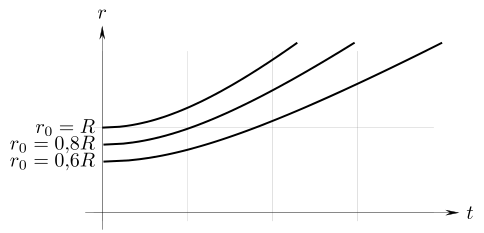
\includegraphics[width=0.5\textwidth]{images/png/sphere1.png}
\end{figure}
\\
Плотность зарядов можно найти, определяя для каждого из слоёв, между которыми находится заряд $dq$, толщина между слоями $dr_0$, в момент времени $t$ соответствующее расстояние между слоями:
$dr$:
\[
\rho = \frac{1}{4\pi r^2} \frac{dq}{dr},
\]
где $dr$ определяется $dr_0$, а $dt = 0$. В результате:
\[
	f'\left(\frac{r}{r_0}\right) \frac{dr}{r_0} = f'\left(\frac{r}{r_0}\right) \frac{r dr_0}{r_0^2} 
\]
\[
	\frac{dr}{r} = \frac{dr_0}{r_0}
\]
\[
	\rho = \frac{Q}{4\pi R^3/3} \left(\frac{r_0}{r}\right)^3 = \rho_0 \left(f^{-1}\left(\sqrt{
		\frac{2\alpha k Q}{R^{3}} } t\right)\right)^{-3}
\]
То есть $\rho$ зависит только от времени и не зависит от расстояния, что означает, что шар всегда однороден.

\textit{Второй метод}.

С точки зрения уравнений Максвелла в сферически-симметричном случае:
\[
	\begin{aligned}
		& \begin{vmatrix}
			\cfrac{1}{r^2 \sin \theta} \,\vec{e}_r & \cfrac{1}{r \sin \theta}\, \vec{e}_\theta & \cfrac{1}{r} \, \vec{e}_\alpha \\
			\df{r} & 0 & 0 \\
			E_r & r E_\theta & r \sin \theta E_\alpha
		\end{vmatrix}
		= 
		- \dff{\vec{B}}{t} \\
		& \begin{vmatrix}
		\cfrac{1}{r^2 \sin \theta} \,\vec{e}_r & \cfrac{1}{r \sin \theta}\, \vec{e}_\theta & \cfrac{1}{r} \, \vec{e}_\alpha \\
		\df{r} & 0 & 0 \\
		B_r & r B_\theta & r \sin \theta B_\alpha
		\end{vmatrix}
		= 
		\mu_0 \rho \vec{v} + \frac{1}{c^2} \dff{\vec{E}}{t} \\
		& \frac{1}{r^2} \df{r} \left( r^2 E_r\right) = \frac{\rho}{\varepsilon_0} \\ 
		& \frac{1}{r^2} \df{r} \left( r^2 B_r\right) = 0 \\
		& \left(\dff{\vec{v}}{t} + \vec{v}\cdot\nabla\vec{v}\right) = A \left(\vec{E} + 
		\begin{vmatrix}
		\vec{e}_r & \vec{e}_\theta & \vec{e}_\alpha \\
		v_r & v_\theta & v_\alpha \\
		B_r & B_\theta & B_\alpha
		\end{vmatrix} \right)
	\end{aligned}
	\Rightarrow
	\begin{aligned}
		& \dff{B_r}{t} = 0 \\
		& \dff{B_\theta}{t} = \frac{1}{r} \df{r} \left( r E_\alpha\right) \\
		& \dff{B_\alpha}{t} = - \frac{1}{r} \df{r} \left( r E_\theta\right) \\
		& \dff{E_r}{t} = - \frac{\rho v_r}{\varepsilon_0} \\
		& \dff{E_\theta}{t} = - c^2 \frac{1}{r} \df{r} \left( r B_\alpha\right) - \frac{\rho v_\theta}{\varepsilon_0} \\
		& \dff{E_\alpha}{t} = c^2\frac{1}{r} \df{r} \left( r B_\theta\right) - \frac{\rho v_\alpha}{\varepsilon_0}\\
		& \frac{1}{r^2} \df{r} \left( r^2 E_r\right) = \frac{\rho}{\varepsilon_0} \\ 
		& \frac{1}{r^2} \df{r} \left( r^2 B_r\right) = 0 \\
		& \dff{v_r}{t} = - v_r\dff{v_r}{r} + A\left(E_r + v_\theta B_\alpha - v_\alpha B_\theta\right) \\
		& \dff{v_\theta}{t} = - v_r\dff{v_\theta}{r} + A\left(E_\theta + v_\alpha B_r - v_r B_\alpha\right) \\
		& \dff{v_\alpha}{t} = - v_r\dff{v_\alpha}{r} + A\left(E_\alpha + v_r B_\theta - v_\theta B_r\right) \\
	\end{aligned}
\] 
Если в начальный момент времени:
\[
	E_\alpha, E_\theta, B_r, B_\alpha, B_\theta, v_\theta, v_\alpha, v_r = 0,
\]
то как следует из системы уравнений первого порядка по времени, во все следующие моменты времени:
\[
	E_\alpha, E_\theta, B_r, B_\alpha, B_\theta, v_\theta, v_\alpha = 0,
\]
Остаётся система из трёх уравнений:
\[
	\begin{aligned}
	& \dff{E_r}{t} = - \frac{\rho v_r}{\varepsilon_0} \\
	& \frac{1}{r^2} \df{r} \left( r^2 E_r\right) = \frac{\rho}{\varepsilon_0} \\
	& \dff{v_r}{t} = - v_r\dff{v_r}{r} + A E_r
	\end{aligned}
\]
Отсюда легко получить систему:
\[
	\begin{aligned}
	& \dff{r^2 E_r}{t} + v_r \df{r} \left( r^2 E_r\right) = 0 \\
	& \dff{v_r}{t} + v_r\dff{v_r}{r} = A E_r
	\end{aligned}
\]
Как её решать? Методом характеристик. Все уравнения имеют один и тот же вид и представляют собой уравнения переноса. Скорость переноса $v_r$. Система в методе характеристик:
\[
	\begin{aligned}
	& \Dff{r}{t} = v_r \\
	& \Dff{(r^2 E_r)}{t} = 0 \\
	& \Dff{v_r}{t} = A E_r
	\end{aligned}
\]
Из второго уравнения следует, что:
\[
	E_r = \frac{E_r(0) r_0^2}{r^2} = k\frac{r_0^3}{R^3 r^2} Q = k \frac{q}{r^2}
\]
И система сводится к системе из предыдущего метода.

\section{Влияние гравитации поля на заряженный шар}

Поле имеет энергию и следовательно массу. Резонно предположить, что эта масса должна участвовать в гравитационных взаимодействиях и гравитация поля должна влиять на движение заряженной среды. Попробуем это учесть.

В сферически симметричном случае массу поля, ограниченная сферой радиуса $r(r_0, t)$, можно найти из выражения:
\[
	m = \frac{\varepsilon_0}{2c^2} \int\limits_0^{r(r_0, t)} E_r^2 4 \pi r^2 dr = 
	\frac{4\pi k^2 \varepsilon_0 Q^2}{2c^2 R^6} \int\limits_0^{r_0} \frac{r_0^6}{r^2} \dff{r}{r_0} dr_0 =
	\frac{k Q^2}{2c^2 R^6} \int\limits_0^{r_0} \frac{r_0^6}{r^2} \dff{r}{r_0} dr_0
\]

Будем считать, что гравитация Ньютонова, случай нерелятивистский, плотность заряда и плотность массы пропорциональны:
\[
	\alpha \rho = \rho_m
\]
Тогда получим уравнения движения:
\[
	\Dff{v_r}{t} = (A + G \alpha / k) k\frac{r_0^3}{R^3 r^2} Q + \frac{k Q^2}{2c^2 R^6} \int\limits_0^{r_0} \frac{r_0^6}{r^2} \dff{r}{r_0} dr_0
\]


\section{Метод характеристик для уравнений Максвелла}

Метод характеристик удобно применять для среды, описываемой уравнениями гидродинамики. Система уравнений Максвелла и второй закон Ньютона для заряженной жидкости с отношением заряда к массе для частицы среды $A$:
\[
	\begin{aligned}
	& \div \vec{E} = \frac{\rho}{\varepsilon_0} \\
	& \rot \vec{E} = - \dff{\vec{B}}{t}\\
	& \div \vec{B} = 0 \\
	& \rot \vec{B} = \mu_0 \rho \vec{v} + \frac{1}{c^2} \dff{E}{t} \\
	& \dff{\vec{v}}{t} + (\vec{v}\cdot\nabla) \vec{v} = \vec{a}(A(\vec{E} + \vec{v}\times\vec{B}))
	\end{aligned}
	\Rightarrow
	\begin{aligned}
	& \Dff{\vec{E}}{t} = c^2 \rot \vec{B} - \vec{v} \div \vec{E} + (\vec{v} \cdot \nabla) \vec{E} \\
	& \Dff{\vec{B}}{t} = - \rot \vec{E} + (\vec{v} \cdot \nabla) \vec{B} \\
	& \Dff{\vec{v}}{t} = \vec{a}(A(\vec{E} + \vec{v}\times\vec{B})) \\
	& \Dff{\vec{r}}{t} = \vec{v}
	\end{aligned}
\] 
\[
	\begin{aligned}
	& \Dff{\vec{E}}{t} = c^2 \nabla_B \times \vec{B} - \vec{v} (\nabla_E \cdot \vec{E}) + (\vec{v} \cdot \nabla_E) \vec{E} =
		c^2 \nabla_B \times \vec{B} - \nabla_E \times (\vec{v} \times \vec{E}) =
		c^2 \nabla_{E, B} \times \left(\vec{B} - \frac{\vec{v}}{c^2} \times \vec{E}\right) \\
	& \Dff{\vec{B}}{t} = -  \nabla_E \times \vec{E} - \vec{v} (\nabla_B \cdot \vec{B}) + (\vec{v} \cdot \nabla_B) \vec{B} =
		- \nabla_E \times \vec{E} - \nabla_B \times (\vec{v} \times \vec{B}) =
		- \nabla_{E, B} \times \left(\vec{E} + \vec{v} \times \vec{B}\right) \\
	& \Dff{\vec{v}}{t} = \vec{a}(A(\vec{E} + \vec{v}\times\vec{B})) \\
	& \Dff{\vec{r}}{t} = \vec{v}
	\end{aligned}
\]
Последняя система интересна тем, что вскрывает некоторые внутренние связи, но предыдущая система лучше поддаётся анализу. Итак,
\[
	\begin{aligned}
	& \Dff{\vec{E}}{t} = c^2 \rot \vec{B} - \vec{v} \div \vec{E} + (\vec{v} \cdot \nabla) \vec{E} \\
	& \Dff{\vec{B}}{t} = - \rot \vec{E} + (\vec{v} \cdot \nabla) \vec{B} \\
	& \Dff{\vec{v}}{t} = \vec{a}(A(\vec{E} + \vec{v}\times\vec{B})) \\
	& \Dff{\vec{r}}{t} = \vec{v}
	\end{aligned}
\]
Начальные условия:
\[
	\vec{E}(\vec{r}_0, t_0), \quad \vec{B}(\vec{r}_0, t_0),  \quad\vec{v}(\vec{r}_0, t_0), \quad \vec{r}(t_0) = \vec{r}_0
\]
Решением системы будут выражения:
\[
	\vec{E}(\vec{r}_0, t), \quad \vec{B}(\vec{r}_0, t),  \quad\vec{v}(\vec{r}_0, t), \quad \vec{r}(\vec{r}_0, t)
\]
Здесь $\vec{r}_0$ аналог постоянной интегрирования. Первые три выражения показывают как меняется электромагнитные поля и поле скоростей в различные моменты времени вдоль характеристики. Выбирая в качестве $\vec{r}_0$ все точки пространства, можно получить поле во всём пространстве в различные моменты времени.
\section{Весёлые интегралы}
Произвольные постоянные в неопределённых интегралах далее опущены.
\begin{enumerate}
	\item 
	\[
		\int \frac{dx}{\sqrt{x^2 + 1}} = \mathrm{arsh\,}x = \ln |x + \sqrt{x^2 + 1}|
	\]
	\item
	\[
		\int \sqrt{x^2 + 1} dx = 
		x \sqrt{x^2 + 1} - \int \frac{x^2}{\sqrt{x^2 + 1}}dx =
		x \sqrt{x^2 + 1} - \int \sqrt{x^2 + 1}dx + \int \frac{dx}{\sqrt{x^2 + 1}}
	\]
	\[
		\Rightarrow \quad
		\int \sqrt{x^2 + 1} dx = \frac{x \sqrt{x^2 + 1} + \ln |x + \sqrt{x^2 + 1}|}{2}
	\]
	\item
	\[
		\int \frac{\sqrt{x}}{\sqrt{x-1}} dx = 
		\int 2 \sqrt{x} d\sqrt{x-1} =
		[\sqrt{x - 1} = p]
		= 2 \int \sqrt{p^2 + 1} dp = 
		\sqrt{x} \sqrt{x-1}+ \ln |\sqrt{x - 1} + \sqrt{x}|
	\]
	\item
	\[
		\int \frac{x\,dx}{\sqrt{px^2 - ax - b}} = 
		\frac{1}{\sqrt{p}} \int \frac{\Big(x - \cfrac{a}{2p} + \cfrac{a}{2p}\Big)\,dx}{\sqrt{\Big(x - \cfrac{a}{2p}\Big)^2 - \Big(\cfrac{a^2}{4p^2} + \cfrac{b}{p}\Big)}}
		= \frac{1}{\sqrt{p}} \sqrt{\Big(x - \cfrac{a}{2p}\Big)^2 - \Big(\cfrac{a^2}{4p^2} + \cfrac{b}{p}\Big)} + 
		\frac{1}{\sqrt{p}} \cfrac{a}{2p} \,\mathrm{arch\,} \frac{x - \cfrac{a}{2p}}{\sqrt{\cfrac{a^2}{4p^2} + \cfrac{b}{p}}}
	\]
	\item
	\[
		\int\limits_a^b |x| dx = 
		\begin{cases}
		\frac{b^2 - a^2}{2}, & 0 < a < b \\
		\frac{a^2 + b^2}{2}, & a < 0 < b \\
		\frac{a^2 - b^2}{2}, & a < b < 0
		\end{cases}
		=
		\frac{\sign(b) b^2 - \sign(a) a^2}{2}
	\]
	\[
		\int |x| dx = \int x \sign (x) dx = \sign (x) \frac{x^2}{2}
	\]
	\[
		\int x^n \sign (x) dx = \sign (x) \frac{x^{n+1}}{n + 1}
	\]
	\item
	\[
		\int\limits_{-\infty}^\infty\int\limits_{-\infty}^\infty e^{-x^2 - y^2} dx dy =
		2\pi \int\limits_0^\infty r e^{-r^2} dr = - \pi e^{-r^2} \Big|_0^\infty = \pi 	
	\]
	\[
		\int\limits_{-\infty}^{\infty} e^{-x^2} dx = \sqrt{\pi}
	\]
	\item 
	\[
		\Gamma(s) = \int\limits_0^\infty x^{s - 1} e^{-x} dx = 
		-x^{s-1} e^{-x} \Big|_0^\infty + (s - 1) \int\limits_0^\infty x^{s - 2} e^{-x} dx = (s - 1) \Gamma (s - 1)
	\]
	\[
		\Gamma(n) = (n - 1)!
	\]
	\[
		\Gamma(1/2) = \int\limits_0^\infty x^{-1/2} e^{-x} dx = 2 \int\limits_0^\infty e^{-x} dx^{1/2} =
		2 \int\limits_0^\infty e^{-t^2} dt = \int\limits_{-\infty}^\infty e^{-t^2} dt = \sqrt{\pi}
	\]
	\[
		\Gamma((n + 1)/2) = \frac{(n - 1)(n - 3)...(n - 2p - 1)}{2^{p+1}} \Gamma((n - 2p - 1)/2) =
		\begin{cases}
		\frac{(n - 1)!!}{2^{n/2}} \sqrt{\pi} & \text{$n$ -- чётное} \\
		\frac{(n - 1)!!}{2^{(n - 1)/2}} & \text{$n$ -- нечётное}
		\end{cases} 
	\]
	\[
		\frac{\Gamma\left(\frac{n + 1}{2}\right)}{\Gamma\left(\frac{n}{2}\right)}
		=
		\begin{cases}
		\frac{(n - 1)!! 2^{(n - 2)/2}}{(n - 2)!! 2^{n/2}} \sqrt{\pi} & \text{$n$ -- чётное} \\
		\frac{(n - 1)!! 2^{(n - 1)/2}}{(n - 2)!! 2^{(n - 1)/2}} \frac{1}{\sqrt{\pi}} & \text{$n$ -- нечётное}
		\end{cases}
		=
		\begin{cases}
		\frac{(n - 1)!!}{(n - 2)!!} \frac{\sqrt{\pi}}{2} & \text{$n$ -- чётное} \\
		\frac{(n - 1)!!}{(n - 2)!!} \frac{1}{\sqrt{\pi}} & \text{$n$ -- нечётное}
		\end{cases}
	\]
	\[
		\frac{\Gamma\left(\frac{n + 1}{2}\right)}{\Gamma\left(\frac{n + 2}{2}\right)}
		=
		\begin{cases}
		\frac{(n - 1)!!}{n!!} \sqrt{\pi} & \text{$n$ -- чётное} \\
		\frac{(n - 1)!!}{n!!} \frac{2}{\sqrt{\pi}} & \text{$n$ -- нечётное}
		\end{cases}
	\]
	\item
	\[
		I_n = \int\limits_0^\pi \sin^n x \, dx = - \cos x \sin^{n - 1} x \Big|_0^\pi + (n - 1) \int\limits_0^\pi \sin^{n - 2} x \cos^2 x \, dx = 
		(n - 1) I_{n - 2} - (n - 1) I_n 
	\] 
	\[
		I_n = \frac{n - 1}{n} I_{n - 2} = \frac{(n - 1)(n - 3)...(n - 2p +  1)}{n(n - 2)...(n - 2p + 2)} I_{n - 2p} =
		\begin{cases}
		\frac{(n - 1)!!}{n!!} \pi  & \text{$n$ -- чётное}\\
		\frac{(n - 1)!!}{n!!} 2 & \text{$n$ -- нечётное}
		\end{cases}
		=
		\frac{\Gamma\left(\frac{n + 1}{2}\right)}{\Gamma\left(\frac{n + 2}{2}\right)} \sqrt{\pi}
	\]
	\item
	\[
		\delta(x) = \frac{1}{2\pi} \int\limits_{-\infty}^{\infty} e^{ikx} dk = \frac{1}{\pi} \int\limits_{0}^{\infty} \cos (kx) dk
	\]
	\[
		\int\limits_{0}^{\infty} \cos (kx) dk = \pi \delta(x)
	\]
	\[
		\int\limits_{0}^{\infty} \sin (kx) dk = [kx = k'x + \pi/2] = \int\limits_{-\frac{\pi}{2x}}^{\infty} \cos (k'x) dk' =
		\pi \delta(x) - \int\limits_{-\frac{\pi}{2x}}^{0} \cos (k'x) dk' = 
		\pi \delta(x) - \frac{\sin (k'x)}{x} \Big|_{-\frac{\pi}{2x}}^0 = 
		\pi \delta(x) - \frac{1}{x}
	\]
	\item 
	\[
		\pi \delta^{(2n+1)}(x) = (-1)^{n + 1} \int\limits_{0}^{\infty} k^{2n + 1} \sin (kx) dk
	\]
	\[
		\pi \delta^{(2n)}(x) - (2n)! \frac{1}{x^{2n+1}} = (-1)^{n} \int\limits_{0}^{\infty} k^{2n} \sin (kx) dk
	\]
	\[
		\int\limits_{0}^{\infty} k^{2n + 1} \sin (kx) dk = (-1)^{n + 1} \pi \delta^{(2n+1)}(x)
	\]
	\[
		\int\limits_{0}^{\infty} k^{2n} \sin (kx) dk = (-1)^{n} \pi \delta^{(2n)}(x) - (-1)^{n} (2n)! \frac{1}{x^{2n+1}}
	\]
	\[
		\int\limits_0^\infty e^{ikx} dk = \pi (1 + i) \delta(x) - \frac{i}{x}
	\]
	\[
		\int\limits_0^\infty k^n e^{ikx} dk = \pi \frac{(1 + i)}{i^n} \delta^{(n)}(x) - \frac{i(-1)^n}{i^n} \frac{n!}{x^{n+1}} =
		\pi (1 + i) (-i)^n \delta^{(n)}(x) - i^{n+1} \frac{n!}{x^{n+1}}
	\]
	\item
	\[
		\begin{gathered}
		I_n(\alpha) = \int\limits_0^\pi e^{i\alpha \cos \theta} \sin^n \theta \, d\theta = - \frac{1}{i\alpha} \int\limits_0^\pi  \sin^{n - 1} \theta \, de^{i\alpha \cos \theta} 
		=
		\frac{n - 1}{i\alpha} \int\limits_0^\pi  \sin^{n - 2} \theta \cos \theta \, e^{i\alpha \cos \theta} d\theta
		= \\ =
		- \frac{n - 1}{\alpha} \frac{\partial}{\partial \alpha} \int\limits_0^\pi  \sin^{n - 2} \theta \, e^{i\alpha \cos \theta} d\theta
		=
		- \frac{n - 1}{\alpha} \frac{\partial I_{n - 2}}{\partial \alpha} 
		=
		(-1)^k (n - 1)(n - 3)(n - 5)\cdot\ldots\cdot(n - (2k - 1)) \left(\frac{1}{\alpha} \frac{\partial}{\partial \alpha} \right)^k I_{n - 2k}
		= \\ =
		\begin{cases}
			(-1)^k (2k)!! \left(\dfrac{1}{\alpha} \dfrac{\partial}{\partial \alpha} \right)^k I_{1} & n = 2k + 1 \\
			(-1)^k (2k - 1)!! \left(\dfrac{1}{\alpha} \dfrac{\partial}{\partial \alpha} \right)^k I_{0} & n = 2k
		\end{cases}
		\end{gathered}
	\]
	\[
		\begin{gathered}
		I_1(\alpha) =
		\int\limits_0^\pi e^{i\alpha \cos \theta} \sin \theta \, d\theta
		=
		\int\limits_0^\pi 
		\left(
			J_0(\alpha) + 2\sum_{p = 1}^{\infty} i^p J_p(\alpha) \cos (p\theta) 
		\right)\sin \theta \, d\theta
		= \\ =
		\int\limits_0^\pi 
		\left(
			J_0(\alpha) \sin \theta + \sum_{p = 1}^{\infty} i^p J_p(\alpha) [\sin ((p + 1)\theta) - \sin ((p - 1) \theta)]
		\right)\, d\theta
		=
		2 J_0(\alpha) + \sum_{p = 1}^{\infty} i^p J_p(\alpha) \left[\frac{1 - (-1)^{p + 1}}{p + 1} - \frac{1 - (-1)^{p - 1}}{p - 1}\right]
		= \\ =
		2 J_0(\alpha) - 4 \sum_{p = 1}^{\infty} (-1)^p J_{2p}(\alpha) \frac{1}{4 p^2 - 1}
		= 
		-\frac{e^{i\alpha \cos \theta}}{i\alpha} \Bigg|_0^\pi = \frac{2 \sin \alpha}{\alpha}
		\end{gathered}
	\]
	\[
		I_0 (\alpha) = \int\limits_0^\pi e^{i\alpha \cos \theta} d\theta = \pi J_0(\alpha)
	\]
	Удивительно, но факт -- результат приводится к общему виду. Воспользуемся соотношениями:
	\[
		J_{k + 1/2} (\alpha) = \frac{(-1)^k \alpha^{k + 1/2}}{\sqrt{2\pi}} \left(\dfrac{1}{\alpha} \dfrac{\partial}{\partial \alpha} \right)^k \dfrac{2 \sin \alpha}{\alpha}
		\qquad
		J_{k} (\alpha) = (-1)^k \alpha^k \left(\dfrac{1}{\alpha} \dfrac{\partial}{\partial \alpha} \right)^k J_0(\alpha)
	\]
	\[
		\Gamma \left(\dfrac{n + 1}{2}\right) = 
		\begin{cases}
		\dfrac{(2k - 1)!!}{2^k} \sqrt{\pi} & n = 2k \\
		\dfrac{(2k)!!}{2^k} & n = 2k + 1
		\end{cases}
	\]
	Получаем:
	\[
		I_n(\alpha) = 
		\begin{cases}
		\Gamma \left(\dfrac{n + 1}{2}\right) 2^{k} \frac{\sqrt{2\pi}}{\alpha^{n/2}} J_{k + 1/2} (\alpha) & n = 2k + 1 \\
		\Gamma \left(\dfrac{n + 1}{2}\right) 2^{k} \frac{\sqrt{\pi}}{\alpha^{n/2}}  J_{k} (\alpha)  & n = 2k
		\end{cases}
		=
		\Gamma \left(\dfrac{n + 1}{2}\right) 2^{n/2} \sqrt{\pi} \frac{J_{n/2} (\alpha)}{\alpha^{n/2}}  
	\]
\end{enumerate}

\end{document}